\subsection{Serial Communication}\label{ssec:serialCommunication}

\subsubsection{Definition}\label{sssec:serialCommunicationDefinition}
	\textit{"Embedded electronics is all about interlinking circuits (processors or other integrated circuits) to create a symbiotic system. In order for those individual circuits to swap their information, they must share a common communication protocol"} \cite{sparkfunSerial}.
\par
	Serial communication is a type of communication characterized for transmitting a bit at a time, usualy done at enormous speeds. There are many types of interfaces: USB, UART, Ethernet,.. being the first and the second related to this project.
\par
	The main advantages of serial communication is the number of wires required, the downside is the speed. Whereas for a 8-bit parallel connection just one clock pulse is needed in order to transmit a byte, in a serial communication eight clock pulses are needed to transmit a byte as Figure \ref{fig:serial_vs_parallel_transmission} shows. 

		\begin{figure}[htbp]
			\centering
				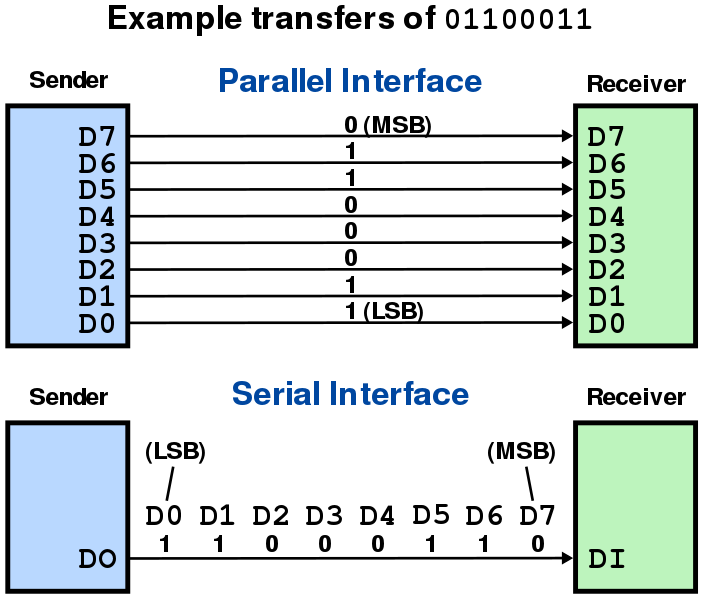
\includegraphics[scale=0.45]{figuras/fig-serial_vs_parallel_transmission}
			\caption{Serial Vs Parallel Transmission \cite{serial_vs_parallel_transmission}}
			\label{fig:serial_vs_parallel_transmission}
		\end{figure}

	However, this was a biggest issue in the past, nowadays with increased clock speeds it is more feasible to implement a more complex software solution (serial) than to jeopardise many MCU IOs for communication (parallel).


\subsubsection{USB}\label{sssec:usb}
	Universal Serial Bus, more commonly known as USB, is a industry standard created to define cables, connectors and protocols for connection, communication and power supply between computers and their peripheral devices \cite{garfinkel1995usb}.
	\par
	There are many specifications in the USB standard, one of than being the USB 1.0. It states that USB cables and connectors must have four wires: a pair of power wires (V$_{BUS}$ and GND) a two wires for differential serial data signals, like Figure \ref{fig:usb2.0-wires}.
	

		\begin{figure}[htbp]
			\centering
				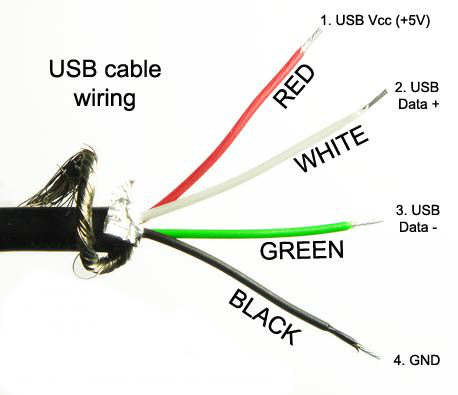
\includegraphics[scale=0.8]{figuras/fig-usb2-0-wires}
			\caption{USB 2.0 Wires \cite{usb2.0-wires}}
			\label{fig:usb2.0-wires}
		\end{figure}

	USB 1.0 specifies data rates of 1.5 Mbit/s (Low-Bandwidth, is mostly used for Human Input Devices (HID) such as keyboards, mouses, joysticks and often the buttons on higher speed devices such as printers or scanners) and 12 Mbit/s (Full-Bandwidth) \cite{specification91}.
	\par
	Differential signaling employs to complementary voltage signals to transmit one information signal, while one wire carries the signal the other carries the inverted signal \cite{diffkinnaird} as Figure \ref{fig:diff-signaling}.

		\begin{figure}[htbp]
			\centering
				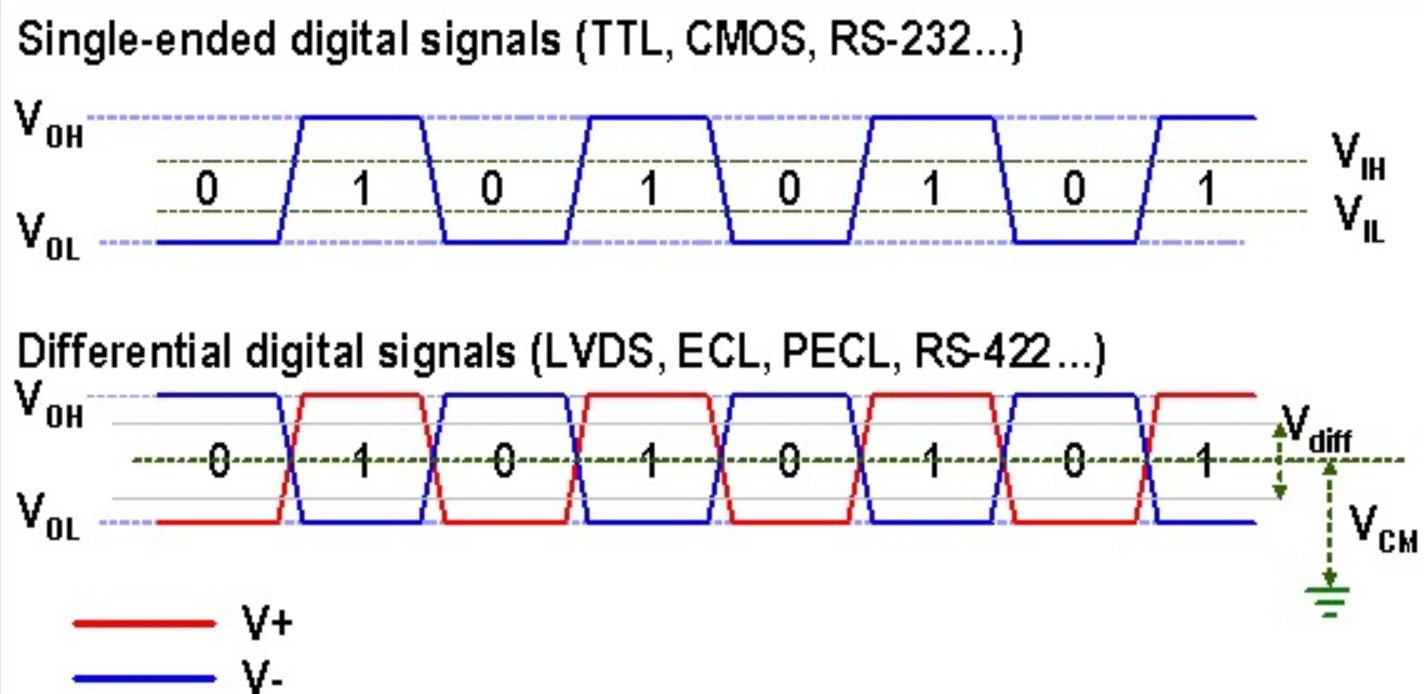
\includegraphics[scale=0.8]{figuras/fig-diff-signaling}
			\caption{What Differential Signaling Is All About \cite{diff-signaling-autodesk}}
			\label{fig:diff-signaling}
		\end{figure}

	Two of the many advantages on differential signaling stated by \cite{pinkle2016dif} are:

	\begin{itemize}
		\item Resistance to EMI: Any interference on the signal will probably affect both signals the same way, so as the receiver responds to the difference between both signals, the receiver will reduce the amplitude of the interference.\label{itm:diff-signaling-emi}
		\item Lower-Voltage Operation: Because of their improved resistance to noise, differential signals can use lower voltages and still maintain adequate SNR. Also, the SNR of differential signaling is automatically increased by a factor of two relative to an equivalent single-ended implementation, because the dynamic range at the differential receiver is twice as high as the dynamic range of each signal within the differential pair.\label{itm:diff-signaling-low-voltage}
	\end{itemize}


\subsubsection{UART}\label{sssec:uart}
	Universal Asynchronous Receiver-Transmitter, more simply UART, is a computer hardware that translates data between parallel and serial forms, it is an integrated circuit that contains both a receiver and a transmitter with individual clocks \cite{futureUart}.
	\par
	UART provides full-duplex communication (data can be transmitted in both directions at the same time \cite{radunovic2011full}) with only three signals \cite{keimUart2016}:
	
	\begin{itemize}
		\item T$_{X}$: Transmitted Serial Data.
		\item R$_{X}$: Received Serial Data.
		\item Ground.
	\end{itemize}

	Figure \ref{fig:uart-connection} shows how two devices UARTs are connected.

		\begin{figure}[htbp]
			\centering
				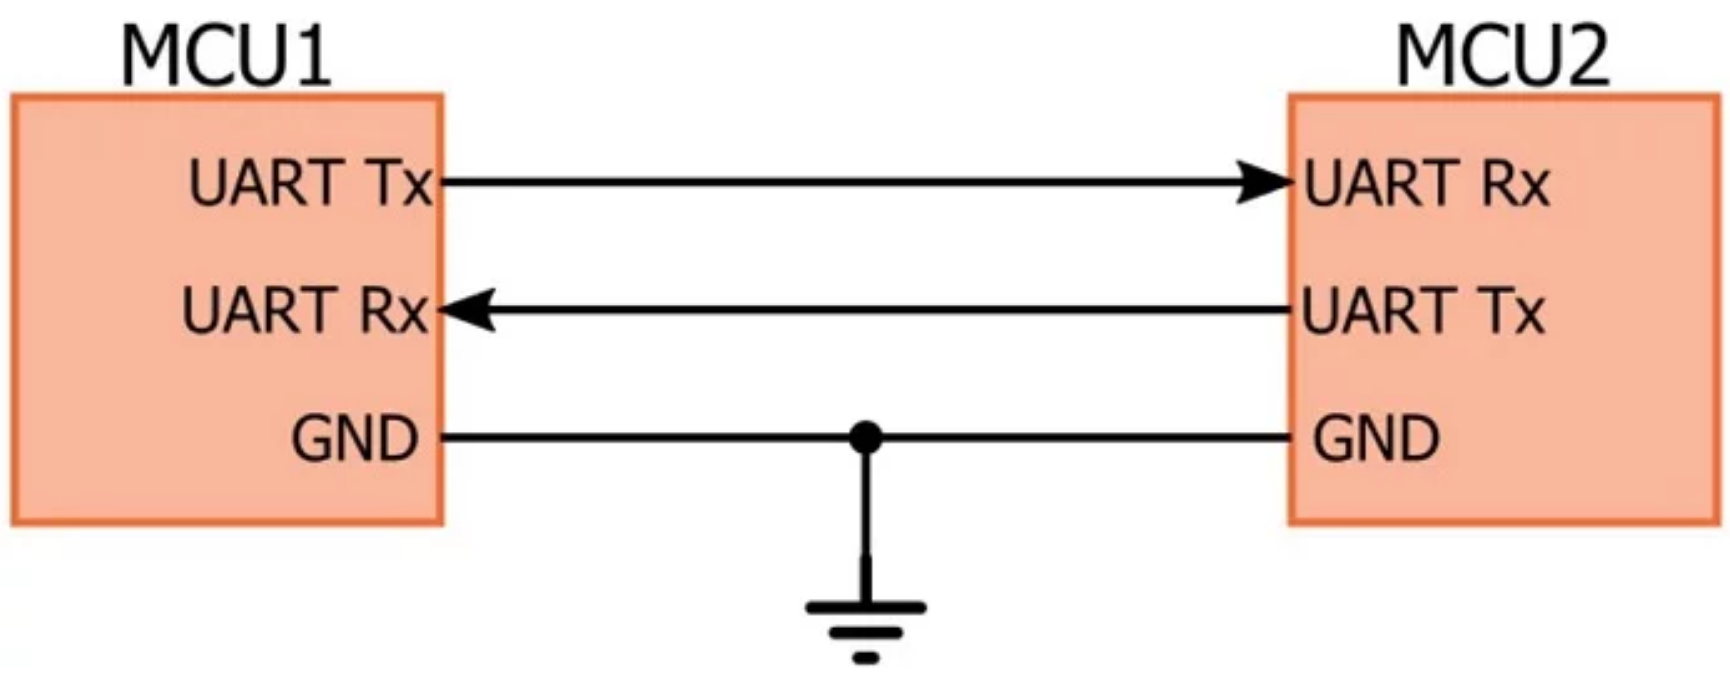
\includegraphics[scale=0.8]{figuras/fig-uart-connection}
			\caption{UART connection \cite{uart-connection}}
			\label{fig:uart-connection}
		\end{figure}	

	UART signals have a start bit (used to indicate when a transmission in starting), stop bit (used to indicated when a transmission has finished) and a parity bit, meaning that in order to transmit a byte, 11 bits of data are required, whereas to transmit two bytes 20 bits are required. The parity bit is transmitted at the end of each byte Other important characteristic of a UART hardware is Baud Rate, being the aproximate rate measured in bits/second at which data can be transfered \cite{keimUart2016}.
